\section{Design der Controller}
\subsection{Pendelidentifikation}
Beim Starten des Programmes zur Regelung des Pendels wird zunächst identifiziert, um welche Pendelaufbaus es sich handelt. Es wird dabei zwischen zwei zuvor definierten Pedenlarmlängen unterschieden.
Für die Identifikation wird wird durch den Motor ein kurzer Impuls auf das Pendel gegeben. 

\colorbox{yellow}{Weiterschreiben}
Je nachdem, welches Pendel auf diese Weise erkannt wurde, werden die entsprechenden Modelldaten geladen und für die Regelung verwendet.

\subsection{Soft-Switch}
Um den Übergang zwischen dem Catcher und dem stabilisierenden Controller möglichst weich zu gestalten, wurde ein Soft-Switch implementiert.

Ziel dieses Switches ist es, extreme Sprünge des Controllerausgangssignals beim Umschalten zwischen den Controllern zu verhindern, selbst wenn die einzelnen Regelsignale des Catchers und des Stabilisierers sehr weit auseinander liegen.
\colorbox{yellow}{Stabilisierer gegen kleine Störungen}
\begin{figure}[htbp]
	\centering	
	\label{fig.furuta-schematic}
	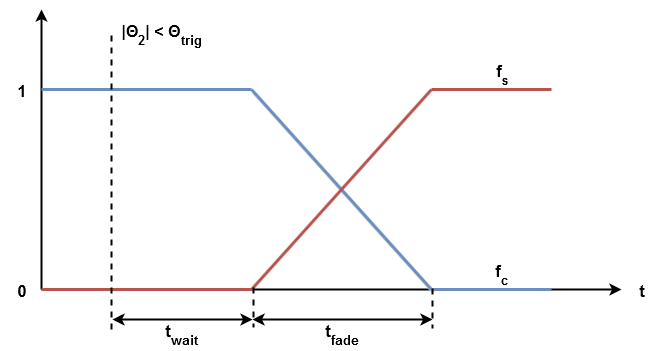
\includegraphics[width=0.8\textwidth]{Grafiken/SoftSwitch.png}
	\caption{Soft-Switch}
\end{figure}

Die Umsetzung erfolgt, indem die einzelnen Regelsignale mit Verstärkungsfaktoren multipliziert werden, die in der Summe genau 1 ergeben, und sich das Gesamtsignal aus den gewichteten Einzelsignalen zusammensetzt.

Zunächst ist lediglich der Catcher aktiv. Dies kommt dadurch zum Ausdruck, dass sein Verstärkungsfaktor $f_c$ den Wert 1 besitzt. Folglich muss der Faktor $f_s$ des Stabilisierers 0 betragen.

Wenn nun der Betrag des Winkels $\theta_2$ für mindestens $t_{wait}$ kleiner als $\theta_{trig}$ ist, beginnt der Crossfader, das Verhältnis der Regelsignale zu verändern.

Während der Faktor des Catchers innerhalb der Zeit $t_{fade}$ linear von 1 auf 0 abfällt, erhöht sich der Faktor des Stabilisierers gegenläufig innherhalb derselben Zeit von 0 auf 1.

Nach Abschluss dieses Vorgangs ist nur noch der Stabilisierer für die Regelung des Pendels zuständig. \\

Wird zu irgendeiner Zeit der Winkel $\theta_{trig}$ überschritten, wird instantan mittels eines Hardswitches der Catcher wieder aktiv geschaltet.

In unserem Controller wurden die Werte wie folgt gewählt:
\begin{eqnarray*}
&& \theta_{trig} = 5^{\circ} \\
&& t_{wait} = 1 s \\
&& t_{fade} = 0.5 s
\end{eqnarray*}
\colorbox{yellow}{Werte überprüfen}


\textit{Hinweis:} Die Funktionsweise dieses Verfahrens ist dabei identisch mit der eines Crossfaders, wie er teilweise beim Übergang zwischen zwei Musikstücken verwendet wird.




